\documentclass[conference]{IEEEtran}
%\IEEEoverridecommandlockouts
% The preceding line is only needed to identify funding in the first footnote. If that is unneeded, please comment it out.
\usepackage{cite}
\usepackage{amsmath,amssymb,amsfonts}
\usepackage{algorithmic}
\usepackage{graphicx}
\usepackage{textcomp}
\usepackage{xcolor}
\usepackage{cuted}
\usepackage{tikz}
\usepackage{pgfplots}


\usetikzlibrary{calc,trees,positioning,arrows,chains,shapes.geometric,%
    decorations.pathreplacing,decorations.pathmorphing,shapes,%
    matrix,shapes.symbols}

\tikzstyle{line} = [draw, -, thick]
\tikzstyle{nodraw} = [draw, fill, circle, minimum width=0pt, inner sep=0pt]
\tikzstyle{box} = [line, rectangle, rounded corners, text centered]

\tikzset{
>=stealth',
  punktchain/.style={
    rectangle, 
    rounded corners, 
    draw=black, very thick,
    text width=2em, 
    minimum height=3em, 
    text centered, 
    on chain},
  line/.style={draw, thick, <-},
  element/.style={
    tape,
    top color=white,
    bottom color=blue!50!black!60!,
    minimum width=1em,
    draw=blue!40!black!90, very thick,
    text width=2em, 
    minimum height=3.5em, 
    text centered, 
    on chain},
  every join/.style={->, thick,shorten >=1pt},
  decoration={brace},
  tuborg/.style={decorate},
  tubnode/.style={midway, right=2pt},
}


\def\BibTeX{{\rm B\kern-.05em{\sc i\kern-.025em b}\kern-.08em
    T\kern-.1667em\lower.7ex\hbox{E}\kern-.125emX}}
\newcommand*\Laplace{\mathop{}\!\mathbin\bigtriangleup}
\begin{document}

\title{Combining checkpointing and data compression\\ for high frequency seismic imaging
}

\author{\IEEEauthorblockN{Navjot Kukreja}
\IEEEauthorblockA{\textit{Department of Earth Science and Engineering} \\
\textit{Imperial College London}\\
London, UK \\
n.kukreja@imperial.ac.uk}
\and
\IEEEauthorblockN{Jan H\"uckelheim}
\IEEEauthorblockA{\textit{Department of Earth Science and Engineering}\\
\textit{Imperial College London}\\
London, UK }
\and
\IEEEauthorblockN{Mathias Louboutin}
\IEEEauthorblockA{\textit{TODO Mathias} \\
\textit{Georgia Institute of Technology}\\
Atlanta, GA, USA\\}
\and
\IEEEauthorblockN{Kaiyuan Hou}
\IEEEauthorblockA{\textit{Department of EECS} \\
\textit{Northwestern University}\\
Evanston, IL, USA \\
}
\and
\IEEEauthorblockN{5\textsuperscript{th} Given Name Surname}
\IEEEauthorblockA{\textit{dept. name of organization (of Aff.)} \\
\textit{name of organization (of Aff.)}\\
City, Country \\
email address}
\and
\IEEEauthorblockN{Gerard Gorman}
\IEEEauthorblockA{\textit{Department of Earth Science and Engineering}\\
\textit{Imperial College London}\\
London, UK }
}

\maketitle

\begin{abstract}
Full-waveform inversion is an adjoint-based optimization problem in seismic
imaging that processes terabytes of data, regularly exceeding the memory
capacity of available computers. Data compression is an effective strategy to
reduce this memory requirement by a certain factor, particularly if some loss in
accuracy is acceptable. A popular alternative is checkpointing, where data is
stored at selected points in time, and values at other times are recomputed as
needed from the last stored state.  This allows arbitrarily large adjoint
computations with limited memory, at the cost of additional recomputations.

In this paper we combine compression and checkpointing for the first
time to compute a realistic full-waveform inversion. The combination of
checkpointing and compression allows
larger adjoint computations compared to using only compression, and
reduces the recomputation overhead significantly compared to using only checkpointing.
\end{abstract}

\begin{IEEEkeywords}
Checkpointing, compression, adjoints, inversion
\end{IEEEkeywords}

\section{Introduction}
Adjoint-based optimization problems typically consist of a simulation that is
run forward in simulation time, producing data that is used in reverse order by
a subsequent adjoint computation that is run backwards in simulation time.
Figure~\ref{fig:dataflow} shows the resulting data flow. Many important
applications in science and engineering have this structure, including
full-waveform inversion (FWI).

In FWI, the propagation of seismic waves through the earth's subsurface is
simulated and compared with data from real-world measurements. The model of the
subsurface is iteratively improved by minimizing the misfit between simulation and
measurement in an adjoint optimization problem.
Figure~\ref{fig:offshore_survey} shows the setup of the real-world experiment that
produces the measurement data~\cite{plessix2006review}. Storing all intermediate
results as required for the data flow shown in Figure~\ref{fig:dataflow} is not
feasible, since this would require tens of terabytes of memory, which is not
commonly available on the machines used to solve these problems. To solve this
problem, a number of strategies are used that are discussed in the following
paragraphs. While this paper uses FWI as a test case, most of these ideas,
including the one presented in this work, are also applicable to other adjoint
optimization problems.

\begin{figure}
\begin{center}
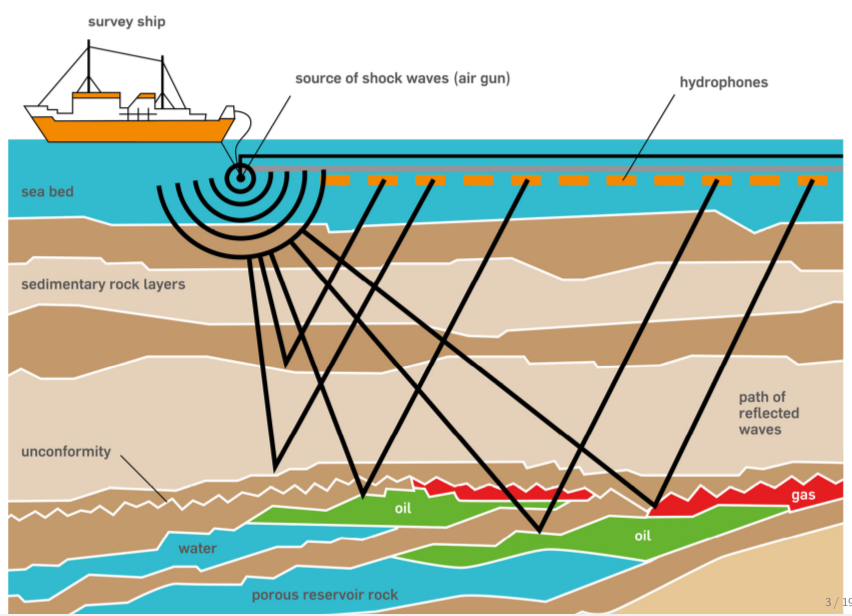
\includegraphics[width=0.8\linewidth]{images/survey-ship-diagram.png}
\end{center}
\caption{Illustration of an offshore seismic survey that collects the input data for FWI}
\label{fig:offshore_survey}
\end{figure}

Domain decomposition is often used not only to distribute the computational
workload across more processors, but also to utilise the large amount of memory
available in distributed systems. While this strategy is very powerful, the
number of compute nodes and therefore the amount of memory that can be used
efficiently is limited, for example by communication overheads that start to
dominate as the domain is split into increasingly small
pieces~\cite{virieux2009seismic}.
Another common strategy in FWI is to only store values at the boundaries of the
domain at each timestep, and reconstruct the rest of the wavefield when
required~\cite{clapp2009reverse,yang2014rtm}.

Checkpointing is yet another strategy to reduce the memory overhead. Only a
subset of the program states during the forward pass is stored (and the rest
discarded).  The discarded data is recomputed when needed by restarting the
forward pass from the last available stored state. The question which states
should be stored and which states should be recomputed to minimize the total
amount of recomputation work has been answerd under certain assumptions with the
Revolve algorithm~\cite{griewank2000algorithm}.  Other authors have subsequently
developed extensions to Revolve that are optimal under less restrictive
assumptions~\cite{wang2009minimal,aupy2016optimal,schanen2016asynchronous}.

\begin{figure*}
\begin{center}
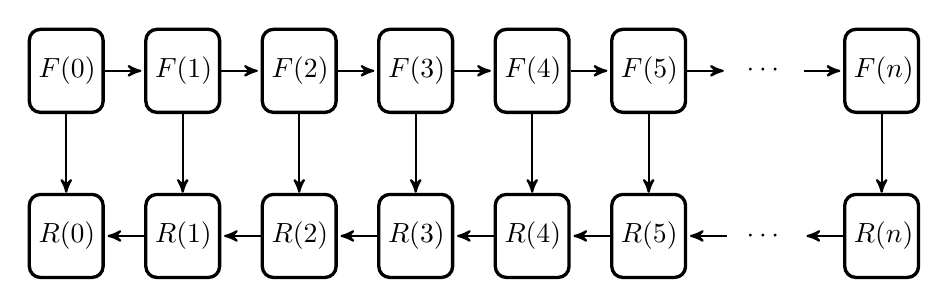
\begin{tikzpicture}
  [node distance=.5cm,
  start chain=1 going right,start chain=2 going left]
     \node[punktchain, join, on chain=1] (t1) {$F(0)$};
     \node[punktchain, join, on chain=1] (t2)      {$F(1)$};
     \node[punktchain, join, on chain=1] (t3)      {$F(2)$};
     \node[punktchain, join, on chain=1] (t4) {$F(3)$};
     \node[punktchain, join, on chain=1] (t5) {$F(4)$};
     \node[punktchain, join, on chain=1] (t6) {$F(5)$};
     \node[punktchain, join, draw=none, on chain=1] (ellipsis1) {$\cdots$};
     \node[punktchain, join, on chain=1] (tn) {$F(n)$};

\node[punktchain, below=1cm of tn, on chain=2] (atn) {$R(n)$};
\node[punktchain, join, draw=none, on chain=2] (ellipsis2) {$\cdots$};
     \node[punktchain, join, on chain=2] (at6)      {$R(5)$};
     \node[punktchain, join, on chain=2] (at5)      {$R(4)$};
     \node[punktchain, join, on chain=2] (at4) {$R(3)$};
     \node[punktchain, join, on chain=2] (at3) {$R(2)$};
     \node[punktchain, join, on chain=2] (at2) {$R(1)$};
     \node[punktchain, join, on chain=2] (at1) {$R(0)$};

\draw[|-,-|,->, thick,] (t1.south) |-+(0,-1em)-| (at1.north);
\draw[|-,-|,->, thick,] (t2.south) |-+(0,-1em)-| (at2.north);
\draw[|-,-|,->, thick,] (t3.south) |-+(0,-1em)-| (at3.north);
\draw[|-,-|,->, thick,] (t4.south) |-+(0,-1em)-| (at4.north);
\draw[|-,-|,->, thick,] (t5.south) |-+(0,-1em)-| (at5.north);
\draw[|-,-|,->, thick,] (t6.south) |-+(0,-1em)-| (at6.north);
\draw[|-,-|,->, thick,] (tn.south) |-+(0,-1em)-| (atn.north);
  \end{tikzpicture}
\end{center}
\caption{The dataflow pattern that is typical of adjoint-based optimization problems}
\label{fig:dataflow}
\end{figure*}


Data compression is also increasingly used to reduce the memory footprint of
scientific applications. General purpose data compression algorithms like Zlib
(which is a part of gzip)~\cite{deutsch1996zlib}, and compression algorithms for
video and image data such as JPEG-2000~\cite{skodras2001jpeg} have been
presented in previous work. More recently, special purpose compression
algorithms for floating-point scientific data have been developed, such as ZFP
or SZ~\cite{Kaklamanis:2012aa,lindstrom2014fixed,di2018efficient}.

Lossless algorithms guarantee that the exact original data can be recovered
during decompression, whereas lossy algorithms introduce an error, but often
guarantee that the error does not exceed certain absolute or relative error
metrics. Typically, lossy compression is more effective in reducing the data
size. Most popular compression packages offer various settings that allow a
tradeoff between compression ratio, accuracy, and compression and decompression
time. In this work we use the ZFP package to perform lossy compresssion.

It is worth noting that another data reduction strategy is to typecast values
into a lower precision format, for example, from double precision to single
precision. This can be seen as a computationally cheap lossy compression
algorithm with a compression ratio of $2$.

Perhaps counterintuitively, compression can not only reduce the memory
footprint, but also speed up an application. Previous work has observed that the
compression and decompression time can be less than the time saved from the
reduction in data that needs to be communicated across MPI nodes or between a
GPU and a host computer~\cite{gpu-compression}.

Another way of using compression to speed up FWI or other adjoint-based methods
is to use it \emph{instead} of checkpointing. If the compression ratio is
sufficient to fit the entire data in memory, checkpointing is no longer
necessary. Previous work has discussed this situation in the context of
computational fluid dynamics~\cite{cyr2015towards} and FWI using compression
method specifically designed for
wavefields~\cite{dalmau2014lossy,boehm2016wavefield}.

In this paper, we extend the previous studies by \emph{combining} checkpointing
and compression. This is obviously useful when the data does not fit in the
available memory even after compression, for example for very large adjoint
problems, or for problems where the required accuracy limits the achievable
compression ratios.

Compared to using only checkpointing without compression, our combined method
often improves performance. This is a consequence of the reduced size of stored
program states, allowing more program states to be stored during the forward
computation. This in turn reduces the amount of recomputation that needs to be
performed. On the other hand, the compression and decompression itself takes
time. We thereforen provide a comprehensive performance model that predicts
whether the combined method is beneficial, that is, whether the time spent
compressing and decompressing is less than the time saved by reduced
recomputations.

We present test cases that use a TODO describe Richter
and TODO describe JLSE/SKX node system, henceforth called Richter and Skylake,
respectively. We discuss performance results for varying error tolerances for
the lossy ZFP compression algorithm ranging from TODO to TODO, and different
types of forward and adjoint computations that vary in their ratio between
compute cost and state size. 

Our aim is to make this discussion independent of the hardware, application and
compression algorithm. We therefore do not discuss whether or not the accuracy
of the decompressed data is sufficient for our application, or whether
other algorithms might achieve a better accuracy/compression tradeoff.

\section{Test case using Devito and pyRevolve}
We use Devito~\cite{devito-api,devito-compiler} to solve forward and adjoint
wave equation problems. Devito is a domain-specific language to enable the
rapid development of finite-difference solvers from a high-level description
of a partial differential equation. The simplest version of the wave
equation is the acoustic wave equation given by
\begin{equation}
m(x)\frac{\partial^2 u(t, x)}{\partial t^2} - \Laplace u(t, x) = q(t, x),
\label{eqn:wave}
\end{equation}
where $m(x) = \frac{1}{c^2(x)}$ is the squared slowness, $c(x)$ the spatially
dependent speed of sound, $u(t, x)$ is the wavefield, $\Laplace u(t, x)$
denotes the laplacian of the wavefield and $q(t, x)$ is a source term.
Some of our experiments in Section TODO are performed using a more accurate
and more complex version of this equation called Tilted Transverse Isotropy
(TTI)~\cite{zhang2011stable}. We leave the TTI equations out of this paper
for brevity. 

The solution to equation~\ref{eqn:wave} forms the forward problem. The adjoint
problem minimizes the misfit between simulated and observed signal given by
\begin{equation}
\min_{m} \phi_s(m) = \frac{1}{2} \left\lVert d_{sim} - d_{obs} \right\rVert_2^2.
\end{equation}
This optimization problem is usually solved using gradient-descent methods,
where the gradient is computed using the adjoint-state method, which involves
the data-flow pattern from figure \ref{fig:dataflow}.

The values of $m(x)$ used in this work are derived from the SEAM Overthrust
model~\cite{aminzadeh1996three} over a grid of $287 \times 881 \times 881$
points, including an absorbing layer of 40 points on each side. The grid spacing
is 25m in space. This is run for 2500 timesteps. The wave field
at the final time is shown in Figure~\ref{fig:uncompressed}, and only this field
was used for the compression experiments in this paper. The uncompressed size of
this single time step field is just under 900MB.

\begin{figure}
\begin{center}
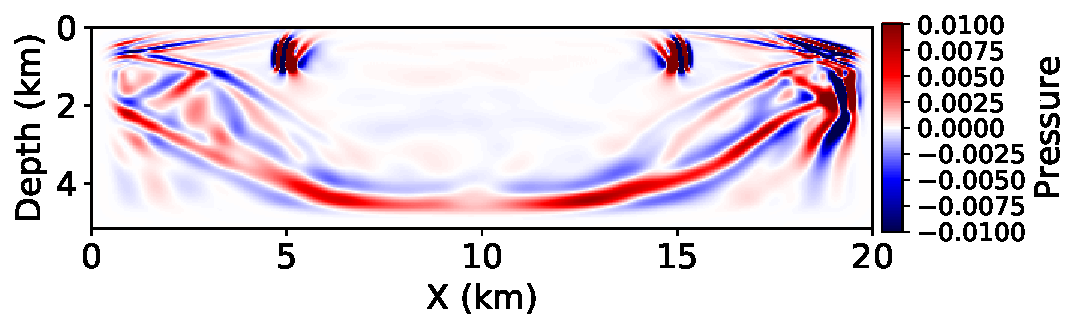
\includegraphics[width=0.8\linewidth]{images/uncompressed.pdf}
\end{center}
\caption{Cross-section of the wavefield used as a reference sample for compression and decompression}
\label{fig:uncompressed}
\end{figure}

To implement Revolve with Devito, we use pyRevolve~\cite{kukreja2018high} which
is a python wrapper for the Revolve algorithm. The performance model in
section~\ref{sec:performance_model} assumes that the implementation is similar
to pyRevolve, which stores a checkpoint by copying a portion of the operator's
working memory to the checkpointing memory and similarly loads a checkpoint by
copying from the checkpointing memory to the operator's working memory. Although
a perfect implementation of checkpointing may be able to avoid these copies, the
overhead attached to these copies can be ignored for an operator that is
sufficiently computationally intensive. However, we include the overheads in the
model to verify this assumption. 

\section{Compression algorithms}
\subsection{Lossless}
For our initial experiments, we used the python package \emph{blosc} \cite{blosc}. It includes implementations for
6 different lossless compression algorithms, namely ZLIB, ZSTD, BLOSCLZ,
LZ4, LZ4HC and Snappy. We did a parameter sweep over all available parameters to find the best-performing combinations. 
The best compression ratio we saw in this study was 1.18x which wasn't very promising.
\subsection{Lossy}
Next we tried lossy compression using ZFP \cite{lindstrom2014fixed}. To use ZFP from python, 
we first wrote a python wrapper over the reference implementation of ZFP, which is in C. We plan to release this wrapper
in the open source community shortly. 

\begin{figure}
\begin{center}
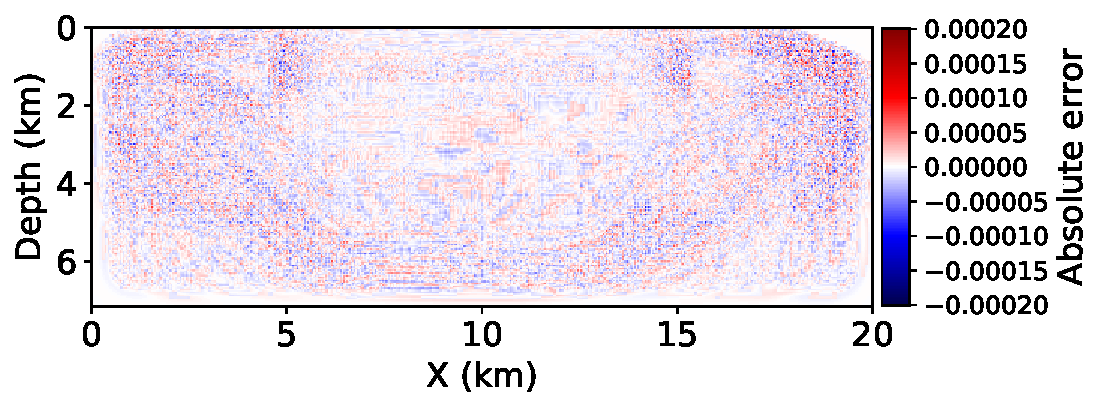
\includegraphics[width=0.8\linewidth]{images/errors.pdf}
\end{center}
\caption{Cross-section of the field that shows errors introduced during compression and decompression using the fixed-tolerance mode}
\label{fig:decompressed_error}
\end{figure}

We tried all three modes of ZFP, namely fixed-tolerance, fixed-precision and fixed-rate modes. Figure \ref{fig:tolerance_cf_plot}
shows the compression ratios we saw for a variety of compression settings for the three modes. As expected, the highest compression efficiency was
observed in the fixed-tolerance mode albeit with highly unpredictable compression ratios. Figure \ref{fig:decompressed_error} shows the
spatial distribution of the error introduced after compression and decompression using fixed-tolerance mode. Since, in our experiments, the time
taken to compress a checkpoint was in the same order of magnitude as the time taken to compute a timestep, we build a
performance model in the next section to evaluate the utility of compression in different scenarios of problem setups and test
platforms.

\begin{figure}
\begin{center}
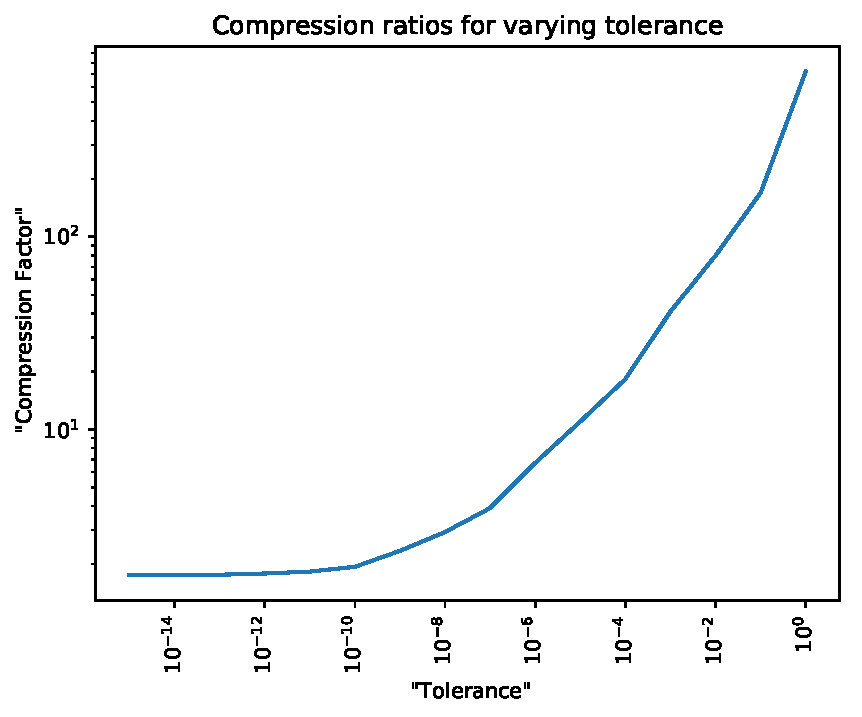
\includegraphics[width=0.8\linewidth]{images/tolerance-cf-richter.pdf}
\end{center}
\caption{Compression ratios achieved on compressing the wavefield}
\label{fig:tolerance_cf_plot}
\end{figure}

\section{Performance model for a combination of Revolve and compression}
\label{sec:performance_model}
We work with the assumption that the computation of a single forward time step takes the same wall time
as the computation of a single reverse time step - calling this $\mathbf{C}$. If the size of a single 
timestep in memory is $\mathbf{S}$ and the simulation involves $\mathbf{N}$ timesteps, the minimum
wall time required to run a single forward-adjoint evaluation is given by:
\begin{equation}
T_N = 2 \cdot \mathbf{C} \cdot \mathbf{N}
\end{equation}
However, this would require $\mathbf{S} \cdot \mathbf{N}$ memory. On a hardware platform where enough memory
is available, this would be the optimal strategy to compute the adjoint solution. 

When the memory available on a system is less than $\mathbf{S} \cdot \mathbf{N}$, Revolve provides
an optimal strategy to solve for the adjoint field by storing a subset of the $\mathbf{N}$ total checkpoints
and recomputing the remaining ones. The overhead introduced by this method can be broken down into
the recomputation overhead $\mathbf{O}_R$ and the storage overhead $\mathbf{O}_S$. The recomputation
overhead is simply the amount of time spent in recomputation, given by:
\begin{equation}
\mathbf{O}_R(N, M) = p(N, M) \cdot \mathbf{C}
\end{equation}
where $p(N, M)$ is the minimum number of recomputed steps from \cite{griewank2000algorithm}, reproduced
here in equation \ref{eqn:recompute}.
\begin{figure*}
\begin{equation}
p(N, M) = \begin{cases}
      N(N-1) /2, & \text{if}\ M=1 \\
      \min\limits_{1<=\widetilde{N}<=N} \{\widetilde{N} + \mathbf{O}_R(\widetilde{N}, M) + \mathbf{O}_R(N-\widetilde{N}, M-1)\}, & \text{if}\ M>1
    \end{cases}
    \label{eqn:recompute}
\end{equation}
\end{figure*}
In equation \ref{eqn:recompute}, M is the number of checkpoints that can be stored in memory. Note that for $M >=N$, $\mathbf{O}_R$
would be zero. For $M < N$, $\mathbf{O}_R$ goes up rather quickly as M is reduced in relation to N. 

In a perfect implementation, the storage overhead $\mathbf{O}_S$ might be zero, since the computation could
be done "in-place", but in practice, checkpoints are generally stored in a separate section of memory and they
need to be transferred to a "computational" section of the memory where the compute is performed, and then
the results copied back to the checkpointing memory. This copying is a common feature of checkpointing
implementations, and might pose a non-trivial overhead in scenarios where the computation is heavily bandwidth-bound. 
This storage overhead is given by:
\begin{equation}
\mathbf{O}_{SR} = \mathbf{N}_W \cdot \frac{\mathbf{S}}{\mathbf{B}} + \mathbf{N}_R \cdot \frac{\mathbf{S}}{\mathbf{B}}
\label{eqn:storage}
\end{equation}
where $\mathbf{N}_W$ is the total number of times Revolve writes checkpoints for a single run, $ \mathbf{N}_R$ 
is the number of times checkpoints are read, and $\mathbf{B}$ is the memory bandwidth of the target system. 

The total time to solution in this scenario becomes:
\begin{equation}
T_R = 2 \cdot \mathbf{C} \cdot \mathbf{N} + \mathbf{O}_R(N, M) + \mathbf{O}_S
\end{equation}

Adding compression to the mix will increase the number of checkpoints available ($M$ in equation \ref{eqn:recompute}),
hence reducing $\mathbf{O}_R$ while adding overheads related to compression and decompression in $\mathbf{O}_S$,
as well as some error introduced by the compression. Assuming that the error remains within the allowed tolerance,
we hypothesize that, at least for some circumstances, the reduction in $\mathbf{O}_R$ should offset the increase in 
$\mathbf{O}_S$, i.e. lead to an overall decrease in the total time to solution ($T$). To build a performance model that
enables us to find the regions where compression pays off, we assume that the compression algorithm behaves uniformly
across the different time steps of the simulation, i.e. that we get the same compression ratio, compression time and 
decompression time, no matter which of the $N$ possible checkpoints we try to compress/decompress. The storage overhead
now becomes:
\begin{equation}
\mathbf{O}_{SR} = \mathbf{N}_W \cdot (\frac{\mathbf{S}}{\mathbf{F}\mathbf{B}} + t_c) + \mathbf{N}_R \cdot (\frac{\mathbf{S}}{\mathbf{F}\mathbf{B}} + t_d)
\end{equation}
where $\mathbf{F}$ is the compression ratio (i.e. the ratio between the uncompressed and compressed checkpoint), and $t_c$
and $t_d$ are compression and decompression times, respectively. At the same time, the recomputation overhead goes down
because $\mathbf{F}$ times more checkpoints are now available.


TODO add figure here that shows memory on x-axis and speedup on y axis. Split into 3 regions. Region 1, 
where Revolve+Compression makes sense, Region 2, where compression would probably not bring in enough benefit, 
and region 3 where compression would enable the computation to be done without revolve. 
\section{Results}


\section{Conclusions and Future work}

What are the problems?

Future work:
\begin{itemize}
\item Acceptable error bounds
\item A posteriori and a priori metrics
\item Relationship between compression error and field error, propagation of errors in forward simulation
\item Relationship between compression error and gradient error in cross-correlation
\item What else?
\end{itemize}

More than 3D fields (use time correlation)

Parallel decompression

Disk checkpointing

\section*{Acknowledgment}

TODO (Acknowledgments for Navjot)

This work was supported by the U.S. Department of Energy, Office of Science,
Office of Advanced Scientific Computing Research, Applied Mathematics and
Computer Science programs under contract number DE-AC02-06CH11357.
We would also like to acknowledge the support from the SINBAD II project and
the member organizations of the SINBAD Consortium.

We gratefully acknowledge the computing resources provided and operated by the
Joint Laboratory for System Evaluation (JLSE) at Argonne National Laboratory.


\bibliographystyle{plain}
\bibliography{compression}

\vfill
\begin{flushright}
\normalsize
\framebox{\parbox{4.8in}{The submitted manuscript has been created by UChicago
Argonne, LLC, Operator of Argonne National Laboratory (`Argonne'). Argonne, a
U.S. Department of Energy Office of Science laboratory, is operated under
Contract No. DE-AC02-06CH11357. The U.S. Government retains for itself, and
others acting on its behalf, a paid-up nonexclusive, irrevocable worldwide
license in said article to reproduce, prepare derivative works, distribute
copies to the public, and perform publicly and display publicly, by or on behalf
of the Government.  The Department of Energy will provide public access to these
results of federally sponsored research in accordance with the DOE Public Access
Plan. \texttt{http://energy.gov/downloads/doe-public-access-plan}.}}
\end{flushright}

\end{document}
